\documentclass[12pt, a4paper]{report}
\usepackage{graphicx, array, amsthm, amssymb, amsmath, algorithm, algpseudocode, float, xcolor, thmtools, thmbox}
\usepackage[english]{babel}

\makeatletter
\renewcommand\thmbox@headstyle[2]{\bfseries #1}
\makeatother
\newtheorem[style=M,bodystyle=\normalfont]{theorem}{Theorem}
\newtheorem[style=M,bodystyle=\normalfont]{corollary}{Corollary}
\newtheorem[style=M,bodystyle=\normalfont]{lemma}{Lemma}
\newtheorem[style=M,bodystyle=\normalfont]{definition}{Definition}


\title{Numerical Analysis \\ \textit{Theory}}
\author{Christian Rossi}
\date{Academic Year 2023-2024}

\begin{document}

\maketitle

\newpage

\begin{abstract}
The topics of the course are:
\begin{itemize}
    \item Floating-point arithmetic: different sources of the computational error; absolute vs relative errors; the floating point representation 
        of real numbers; the round-off unit; the machine epsilon; floating-point operations; over- and under-flow; numerical cancellation.
    \item Numerical approximation of nonlinear equations: the bisection and the Newton methods; the fixed-point iteration; convergence analysis 
        (global and local results); order of convergence; stopping criteria and corresponding reliability; generalization to the system of 
        nonlinear equations (hints).
    \item Numerical approximation of systems of linear equations: direct methods (Gaussian elimination method; LU and Cholesky factorizations; 
        pivoting; sparse systems: Thomas algorithm for tridiagonal systems); iterative methods (the stationary and the dynamic Richardson scheme; 
        Jacobi, Gauss-Seidel, gradient, conjugate gradient methods (hints); choice of the preconditioner; stopping criteria and corresponding 
        reliability); accuracy and stability of the approximation; the condition number of a matrix; over- and under-determined systems: the 
        singular value decomposition (hints).
    \item Numerical approximation of functions and data: Polynomial interpolation (Lagrange form); piecewise interpolation; cubic interpolating 
        splines; least-squares approximation of clouds of data.
    \item Numerical approximation of derivatives: finite difference schemes of the first and second order; the undetermined coefficient method.
    \item Numerical approximation of definite integrals: simple and composite formulas; midpoint, trapezoidal, Cavalieri-Simpson quadrature rules; 
        Gaussian formulas; degree of exactness and order of accuracy of a quadrature rule. 
    \item Numerical approximation of ODEs: the Cauchy problem; one-step methods (forward and backward Euler and Crank-Nicolson schemes); 
        consistency, stability, and convergence (hints).
\end{itemize}
\end{abstract}

\newpage

\tableofcontents

\newpage

\chapter{Introduction}
    \section{Numerical analysis and errors}
    Numerical analysis is the field of mathematics dealing with methods to find the solutions of certain mathematical problems with an electronic 
    calculator. It is the intersection between math and computer science. 

    On the other hand, scientific computing also deals with the model formalization and so it needs also engineering knowledge. 
    \begin{figure}[H]
        \centering
        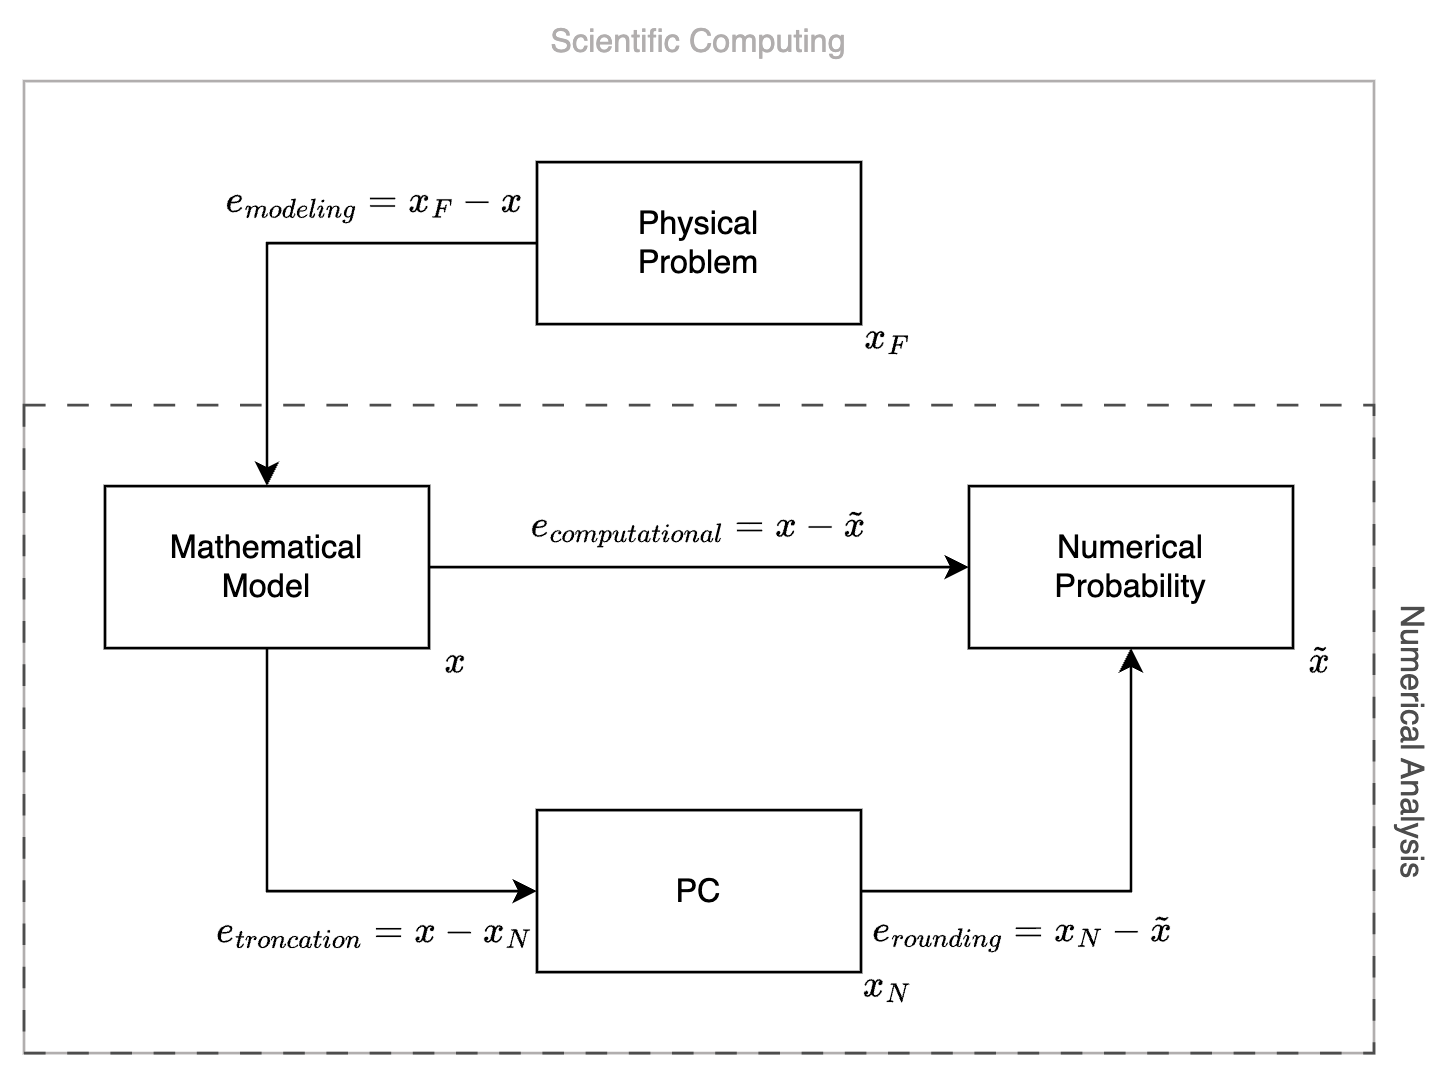
\includegraphics[width=0.75\linewidth]{images/difference.png}
        \caption{Difference between numerical analysis and scientific computing}
    \end{figure}
    As it is possible to see from the diagram every step of the computation have to deal with errors. The possible types of errors are: 
    \begin{itemize}
        \item Absolute: $\left\lvert x - \tilde{x} \right\rvert$
        \item Relative: $\dfrac{\left\lvert x - \tilde{x} \right\rvert}{\left\lvert x \right\rvert}$, where $x \neq 0$
    \end{itemize}
    The relative error is more precise because it compares the error with the measure quantity. 
    \begin{example}
        Let us consider $x=100$ and $\tilde{x}=100.1$. The errors in this case are: 
        \[e_{abs}=\left\lvert x - \tilde{x} \right\rvert=\left\lvert 100 - 100.1 \right\rvert=0.1\]
        \[e_{rel}=\dfrac{\left\lvert x - \tilde{x} \right\rvert}{\left\lvert x \right\rvert}=\dfrac{\left\lvert 100 - 100.1 \right\rvert}{\left\lvert 100 \right\rvert}=0.001\]
        Let us consider $x=0.2$ and $\tilde{x}=0.1$. The errors in this case are: 
        \[e_{abs}=\left\lvert x - \tilde{x} \right\rvert=\left\lvert 0.2 - 0.1 \right\rvert=0.1\]
        \[e_{rel}=\dfrac{\left\lvert x - \tilde{x} \right\rvert}{\left\lvert x \right\rvert}=\dfrac{\left\lvert 0.2 - 0.1 \right\rvert}{\left\lvert 0.2 \right\rvert}=0.5\]
        The result are that the measures have the same absolute error ($10\%$), but the relative error is much grater in the second example ($50\%$ vs $0.1\%$).
        This result proves that the relative error is the most precise.
    \end{example}

    \section{Floating point}
    A calculator can only handle a finite quantity of numbers and compute a finite number of operations. For those reason the set of the real numbers 
    $\mathbb{R}$ is indeed represented by a finite set of machine numbers $\mathbb{F}=\{-\tilde{a}_{min}, \dots , \tilde{a}_{max} \}$ called
    floating points numbers. The function used to find the corresponding value in $\mathbb{F}$ to a number in $\mathbb{R}$ is $fl(x)$ that does an 
    operation called truncation and rounding.

    The set $\mathbb{F}=\mathbb{F}(\beta,t,L,U)$ is characterized by four parameters $\beta,t,L$ and $U$ such that every real number $fl(x) \in \mathbb{F}$ 
    can be written as:
    \[fl(x)=(-1)^s(0.a_1a_2\dots a_t)\beta^e\]
    where:
    \begin{itemize}
        \item $\beta \geq 2$ is the basics, an integer that determines the numeric system. 
        \item $m=(0.a_1a_2\dots a_t)$ is the mantissa.
        \item $e \in \mathbb{Z}$ is the exponent such that $L<e<U$, with $L<0$ and $U>0$. 
        \item $s=\{0,1\}$ is the sign. 
    \end{itemize}
    In the definition of the numbers in the mantissa set we have to set the constraint $a_1 \neq 0$ to ensure the uniqueness of the representation. In this case we say that the number
    is normalized. 

    The set of floating points has the following characteristic values are:
    \begin{itemize}
        \item Machine epsilon, that is the distance between one and the smallest floating point number greater than one, and it is equal to: 
            \[\epsilon_M=\beta^{1-t}\]
        \item Round-off error, that is the relative error that is committed when substituting $x \in \mathbb{R}-\{0\}$ with his corresponding 
            $fl(x) \in \mathbb{F}$. It is limited by: 
            \[\dfrac{\left\lvert x-fl(x) \right\rvert}{\left\lvert x \right\rvert }\leq \dfrac{1}{2}\epsilon_M\]
            where $x \neq 0$.
        \item The biggest and the smallest numbers in the set are found with the formula:
            \[x_{min}=\beta^{L-1}\]
            \[x_{max}=\beta^U(1-\beta^{-t})\]
    \end{itemize}
    \begin{example}
        In MATLAB the floating point set is defined with the following variables:
        \[(\beta=2,t=53,L=-1021,U=1024)\] 
        With the command $eps$ we can find the machine epsilon, that in MATLAB case is:
        \[\epsilon_M=2.22 \cdot 10^{-16}\]
        With the command $realmin$ and $realmax$ we can find the smallest and the largest numbers representable that are equal to:
        \[x_{min}=2.225073858507201 \cdot 10^{-308}\]
        \[x_{max}=1.797693134862316 \cdot 10^{308}\]
    \end{example}
    Since not all the numbers in the $\mathbb{R}$ set are also in the $\mathbb{F}$ set, in the second one there is no continuity. It is possible to 
    demonstrate that while we are increasing the values of the numbers we are also increasing the distance between two consecutive numbers in $\mathbb{F}$.
    \begin{example}
        Let us consider the floating number set $\mathbb{F}(2,2,-1,2)$. The characteristic values of this set are: 
        \begin{itemize}
            \item $\epsilon_M=\beta^{1-t}=0.5$.
            \item $x_{min}=\beta^{L-1}=0.25$.
            \item $x_{max}=\beta^U(1-\beta^t)=3$.
            \item $\#\mathbb{F}=2 \beta^{t-1}(\beta -1)(U-L+1)+1=16$. 
        \end{itemize}
        The exponent can have the values $-1,0,1$ and $2$. The mantissa will be like $(a_1a_2)_{\beta}$ because $t=2$. The possible positive values are
        reported in the figure. 
        \begin{figure}[H]
            \centering
            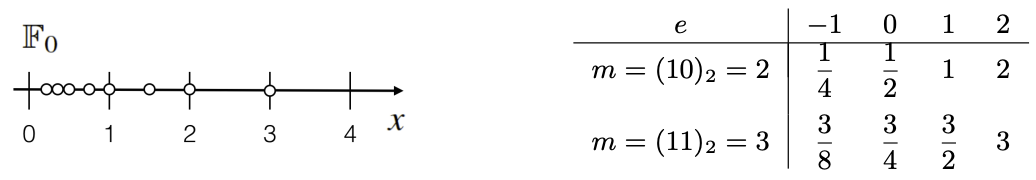
\includegraphics[width=0.9\linewidth]{images/numbers.png}
        \end{figure}
    \end{example}
    The other important aspect is that the passage between the two sets causes the loss of two important properties such as associativity end the 
    neutral number for the sum. 

\newpage 
\chapter{Nonlinear equations}
    \section{Introduction}
    To solve a nonlinear equation $f(x)$ we have to find $\alpha \in \mathbb{R}$ that is a zero of $f$ such that $f(\alpha)=0$.
    \begin{definition}
        The point $\alpha$ is said to be a \emph{zero with multiplicity $m$} if:
        \begin{itemize}
            \item $f(\alpha)=f^{'}(\alpha)=\dots=f^{\left(m-1\right)}(\alpha)=0$.
            \item $f^{\left(m\right)}(\alpha) \neq 0$.
        \end{itemize}
    \end{definition}
    If $m$ is odd the function changes sign across the zero. It does not change the sign if $n$ is even. 

    \section{Iterative methods}
    The set of all the polynomials of degree $n$ is denoted by the symbol $\mathbb{P}_n$ that contains all the polynomial that have a grade less or equal to $n$.
    \begin{theorem}[Abel-Ruffini theorem]
        There is no solution in radicals to general polynomial equations of degree five or higher with arbitrary coefficients. 
    \end{theorem}
    So, to solve polynomials with a degree higher than four we need to use the iterative methods. The general idea of those methods is the following:
    \begin{enumerate}
        \item Select an arbitrary initial value $x^{(0)}$ called initial guess, that is a hypothetical value for $\alpha$.
        \item Use the selected value as an input for a black-box function.
        \item Use the output of the black-box function as the new $x^{(0)}$ and return to point one. 
    \end{enumerate}
    After some iterations (that depends on the chosen method) we will have a set of values $\{ x^{(n)} \}$ convergent such that:
    \[ \lim_{n \rightarrow \infty} = \alpha\]
    and the error related to the value found for $\alpha$ is equal to: 
    \[ \lim_{n \rightarrow \infty}e^n = 0\]
    That implies that the error can be also written as: 
    \[e^n=\alpha-x^{(n)}\]
    All the methods we are going to see constructs a sequence $x^{(1)},x^{(2)},\dots,x^{(n)}$ of numbers that hopefully converges to $\alpha$:
    \[ \lim_{k \rightarrow + \infty} \left\lvert x^{(k)}-\alpha \right\rvert =0\]
    \begin{definition}[order of convergence]
        An iterative method for the approximation of the zero $\alpha$ of the function $f(x)$ is convergent with order $q$ if and only if for $k > k_0$:
        \[\left\lvert x^{(k)} - \alpha \right\rvert \leq c {\left\lvert x^{(k+1)} - \alpha \right\rvert}^q  \]
        We can have two cases:
        \begin{itemize}
            \item If $q=1$ it is called linear convergence and there are the constraint $0<c<1$.
            \item If $q>1$, $c$ can be any positive number grater than zero. 
        \end{itemize}
    \end{definition}

    \section{Stopping conditions}
    The iterative methods needs a stopping criterion. It can be on four possible contitions: 
    \begin{itemize}
        \item On the error, stops if $\left\lvert x^{(k)}-\alpha \right\rvert \leq \epsilon_e$.
        \item On the residual, stops if $\left\lvert f\left(x^{(k)}\right) \right\rvert \leq \epsilon_r$. 
        \item On the step length, stops if $\left\lvert x^{(k)}-x^{(k-1)} \right\rvert \leq \epsilon_s$. 
        \item On the max numbers of iterations, stops if $k \leq k_{max}$. 
    \end{itemize}
    If none of the first three stopping criterions are satisfied, it means that there are no convergence. 




    \section{Bisection method}
    \begin{theorem}[zeros of continuous functions]
        Let $f(x)$ be a continuous function on the interval $I=(a,b)$, that is $f \in C^0([a,b])$. 
        If $f(a)f(b)<0$, then there exists at least one zero $\alpha \in I$ of $f(x)$. 
    \end{theorem}
    Let us assume that exist a unique zero, and let us call it $\alpha$. 
    The strategy of the bisection method is to have the given interval and select a sub-interval where $f$ features a sign change. Following 
    such procedure it is guaranteed that every interval selected this way will contain $\alpha$. The sequence $\{x^{(k)}\}$ of the midpoints of 
    these sub-intervals will inevitably tend to $\alpha$ since the length of the sub-intervals tends to zero as $k$ tends to infinity.
    We have that:
    \[\left\lvert x^{(k)} - \alpha \right\rvert \leq \dfrac{1}{2} \left\lvert b^{(k)}-a^{(k)} \right\rvert \]
    So, since the first part of the equation is similar to the condition on the error, we have that the stopping criterion will be: 
    \[\left\lvert b^{(k)}-a^{(k)} \right\rvert \leq 2 \epsilon_e\]
    Now that we have the tolerance $\epsilon$ we can find that:
    \[k_{min}= \left\lceil {\log_2{\left( \dfrac{\left\lvert b-a \right\rvert}{\epsilon} \right)} - 1}\right\rceil \]
    The inputs for the algorithm are: a function $f \in C(\mathbb{R})$ and an interval $[a,b]$ such that $f(a)f(b) \leq 0$. 
    \begin{algorithm}[H]
        \caption{Algorithm for the bisection method}
            \begin{algorithmic}[1]
                \For {$k=0,1,\dots,n$}
                    \State $x^{(k)}=\dfrac{a+b}{2}$
                    \If {$\left\lvert b^{(k)}-a^{(k)} \right\rvert \leq 2 \epsilon_e$}
                        \State \Return $x^{(k)}$
                    \ElsIf {$f(x^{(k)})f(a) < 0$}
                        \State $b \leftarrow x^{(k)}$
                    \Else 
                        \State $a \leftarrow x^{(k)}$
                    \EndIf
                \EndFor
            \end{algorithmic}
    \end{algorithm}
    The pros are: 
    \begin{itemize}
        \item I can control the maximal error.
        \item Convergence is guaranteed.
        \item Use only evaluation of $f$
    \end{itemize}
    The cons are: 
    \begin{itemize}
        \item Work only if $f$ changes sign. 
        \item Convergence is slow.
    \end{itemize}
   
    \section{Newton method}
    The sign of the given function $f$ at the endpoints of the sub-intervals is the only information exploited by the bisection method. A more efficient method can be constructed 
    by exploiting the values attained by $f$ and its derivative. If $f$ is differentiable we have that: 
    \[y(x)=f(x^{(k)})+f^{'}(x^{(k)})(x-x^{(k)})\]
    provides the equation of the tangent to the curve $(x,f(x))$ at the point $x^{(k)}$. If we pretend that $x^{(k+1)}$ is such that $f(x^{(k+1)})=0$, we obtain:
    \[x^{(k+1)}=x^{(k)}-\dfrac{f(x^{(k)})}{f^{'}(x^{(k)})} \:\:\:\:\:\: k \geq 0\]
    provided $f^{'}(x^{(k)}) \neq 0$. This method is known as Newton's method and corresponds to computing the zero of $f$ locally replacing $f$ by its tangent line. 

    Obviously, this method converges in a single step when $f$ is linear. 

    The Newton method in general does not converges for all possible choices of $x^{(0)}$, but only for those values of $x^{(0)}$ which are sufficiently close to $\alpha$. Since we 
    don't know the value of $\alpha$ a possible initial value $x^{(0)}$ can be obtained by resorting to a few iterations of the bisection method or through an investigation of the 
    graph of $f$. 

    If $f \in C^2(\mathbb{R})$, $f^{'}(\alpha) \neq 0$, and $x^{(0)}$ is taken sufficiently near $\alpha$ the Newton method converges quadratically. In the case of zeros with 
    multiplicity $m$ larger than one Newton method converges linearly. To avoid this degradation it is possible to use the modified Newton method:
    \[x^{(k+1)}=x^{(k)}-m\dfrac{f(x^{(k)})}{f^{'}(x^{(k)})} \:\:\:\:\:\: k \geq 0\]
    provided $f^{'}(x^{(k)}) \neq 0$.

    Another modification to this method is the quasi-Newton method that uses a derivative by finite difference: 
    \[f^{'}(x^{(k)}) \simeq \dfrac{f(x^{(k)}+h)-f(x^{(k)})}{h}\]

    The inputs for the algorithm are: a function $f \in C^1(\mathbb{R})$ and an initial guess $x^{(0)} \in \mathbb{R}$. 
    \begin{algorithm}[H]
        \caption{Algorithm for the basic Newton method}
            \begin{algorithmic}[1]
                \For {$k=0,1,\dots,n$}
                    \State $x^{(k+1)}=x^{(k)}-\dfrac{f(x^{(k)})}{f^{'}(x^{(k)})}$
                    \If {$k>k_{max} \lor \left\lvert x^{(k)}-x^{(k-1)} \right\rvert \leq \epsilon_s \lor \left\lvert f\left(x^{(k+1)}\right) \right\rvert \leq \epsilon_r$}
                        \State \Return $x^{(k+1)}$
                    \EndIf
                \EndFor
            \end{algorithmic}
    \end{algorithm}
    The pros are: 
    \begin{itemize}
        \item Fast convergence. 
        \item Works also for zeros with even multiplicity. 
    \end{itemize}
    The cons are: 
    \begin{itemize}
        \item Require computation of the derivative. 
        \item Choice of the right $x^{(0)}$. 
    \end{itemize}

    \section{Secant method}
    For the computation of the zeros of a function $f$ whose derivative is not available in analytical form, the Newton method cannot be applied. However, we should be able to 
    compute the function $f$ at any arbitrary point, and we could replace the exact value $f^{'}(x^{(k)})$ with an incremental ratio based on previously computed values of $f$. The 
    secant method exploits this strategy and converges super-linearly ($q=1.6$). 

    The inputs for the algorithm are: two initial guesses $x^{(0)} \in \mathbb{R}$ and $x^{(1)} \in \mathbb{R}$. 
    \begin{algorithm}[H]
        \caption{Algorithm for the secant method}
            \begin{algorithmic}[1]
                \For {$k=0,1,\dots,n$}
                    \State $x^{(k+1)}=x^{(k)}-f(x^{(k)})\dfrac{x^{(k)}-x^{(k-1)}}{f(x^{(k)})-f(x^{(k-1)})}$
                    \If {$k>k_{max} \lor \left\lvert x^{(k)}-x^{(k-1)} \right\rvert \leq \epsilon_s \lor \left\lvert f\left(x^{(k+1)}\right) \right\rvert \leq \epsilon_r$}
                        \State \Return $x^{(k+1)}$
                    \EndIf
                \EndFor
            \end{algorithmic}
    \end{algorithm}

    \section{Systems of nonlinear equations}

    \section{Fixed point method}
    Given a function $\phi:[a,b] \rightarrow \mathbb{R}$, find $\alpha \in [a,b]$ such that $\alpha=\phi(\alpha)$. If such an $\alpha$ exists it will be called a fixed point of 
    $\phi$, and it could be computed by the following algorithm: 
    \[x^{(k+1)}=\phi(x^{(k)}) \:\:\:\:\:\: k \geq 0\]
    where $x^{(0)}$ is an initial guess. This algorithm is called fixed point iteration and $\phi$ is said to be the iteration function. 
    \begin{theorem}[Lipschitz continuity]
        \begin{enumerate}
            \item Let us suppose that $\phi(x)$ is continuous in $[a,b]$ and such that $\phi(x) \in [a,b]$ for every $x \in [a,b]$; then, there exists at least a fixed point 
                $\alpha \in [a,b]$.
            \item Moreover, if 
                \[\exists L < 1 \textnormal{such that} \left\lvert \phi(x_1)-\phi(x_2) \right\rvert \leq L\left\lvert x_1-x_2 \right\rvert  \:\:\:\:\:\: \forall x_1,x_2 \in [a,b]\]
                then there exists a unique fixed point $\alpha \in [a,b]$ of $\phi$ and the sequence converges to $\alpha$, for any choice of initial guess $x^{(0)} \in [a,b]$.
        \end{enumerate}
    \end{theorem}
    \begin{proof}[of the first proposition]
        
    \end{proof}
    \begin{proof}[of the second proposition]
        
    \end{proof}
\end{document}